\documentclass[preview]{standalone}

\usepackage{amsmath}
\usepackage{amssymb}
\usepackage{stellar}
\usepackage{definitions}
\usepackage{tikz}
\usepackage{bettelini}

\begin{document}

\id{sequences-functions-limits}
\genpage

\section{Interchange of limits}

\begin{snippettheorem}{uniform-convergence-interchange-limits-theorem}{Interchange of limits under uniform convergence}
    Let \(S\subseteq\realnumbers\), let \(x_0\) be an accumulation point of
    \(S\), and let \(\{f_n\}_{n\in\naturalnumbers}\) be a \sequence of
    \function[functions] \(f_n\colon S\fromto\realnumbers\) converging
    uniformly on \(S\) to \(f\colon S\fromto\realnumbers\). If the finite
    limit
    \[
        A_n=\lim_{x\to x_0}f_n(x)
    \]
    exists for every \(n\in\naturalnumbers\), then both iterated limits exist
    and
    \[
        \lim_{n\to\infty}\lim_{x\to x_0}f_n(x)
        =\lim_{x\to x_0}\lim_{n\to\infty}f_n(x).
    \]
\end{snippettheorem}

\begin{snippetproof}{uniform-convergence-interchange-limits-theorem-proof}{uniform-convergence-interchange-limits-theorem}{Interchange of limits under uniform convergence}
    Define \(A_n=\lim_{x\to x_0}f_n(x)\). By the uniform Cauchy criterion,
    for every \(\varepsilon>0\) there exists \(N\in\naturalnumbers\) such that
    \[
        |f_n(x)-f_m(x)|<\varepsilon,
        \qquad \forall m,n>N,\ \forall x\in S.
    \]
    Letting \(x\to x_0\) gives \(|A_n-A_m|\leq\varepsilon\). Thus
    \(\{A_n\}\) is Cauchy and converges to some \(A\in\realnumbers\).

    It remains to show that \(\lim_{x\to x_0}f(x)=A\). Fix
    \(\varepsilon>0\). Uniform convergence gives \(N_1\) such that
    \[
        |f_n(x)-f(x)|<\frac{\varepsilon}{3}
    \]
    for every \(n>N_1\) and \(x\in S\), while \(A_n\to A\) gives \(N_2\)
    such that \(|A_n-A|<\frac{\varepsilon}{3}\) for every \(n>N_2\).
    Fix \(M>\max\{N_1,N_2\}\). Since \(f_M(x)\to A_M\) as
    \(x\to x_0\), there exists \(\delta>0\) such that
    \[
        |f_M(x)-A_M|<\frac{\varepsilon}{3}
    \]
    whenever \(x\in S\difference\{x_0\}\) and \(|x-x_0|<\delta\).
    Consequently,
    \begin{align*}
        |f(x)-A|
        &\leq |f(x)-f_M(x)|+|f_M(x)-A_M|+|A_M-A|\\
        &<\varepsilon.
    \end{align*}
    Hence \(\lim_{x\to x_0}f(x)=A\), which is the desired equality.
\end{snippetproof}

\begin{snippet}{uniform-convergence-interchange-infinite-limits}
    The same conclusion holds when
    \(\lim_{x\to x_0}f_n(x)=+\infty\) for every \(n\), in which case
    \(\lim_{x\to x_0}f(x)=+\infty\), and analogously for \(-\infty\).
    Finite and infinite cases can be stated uniformly by using neighborhoods
    in the extended real line.
\end{snippet}

\section{Continuity}

\begin{snippetcorollary}{uniform-limit-continuity-corollary}{Uniform limit of continuous functions}
    Let \(S\subseteq\realnumbers\) and let
    \(\{f_n\}_{n\in\naturalnumbers}\) be a \sequence of continuous
    \function[functions] \(f_n\colon S\fromto\realnumbers\). If \(f_n\)
    converges uniformly on \(S\) to \(f\colon S\fromto\realnumbers\), then
    \(f\) is continuous on \(S\). In particular, for every accumulation point
    \(x_0\in S\),
    \[
        \lim_{n\to\infty}\lim_{x\to x_0}f_n(x)
        =\lim_{x\to x_0}\lim_{n\to\infty}f_n(x)=f(x_0).
    \]
\end{snippetcorollary}

\begin{snippetproof}{uniform-limit-continuity-corollary-proof}{uniform-limit-continuity-corollary}{Uniform limit of continuous functions}
    Fix \(x_0\in S\) and \(\varepsilon>0\). Uniform convergence yields an
    index \(N\) such that
    \[
        |f_n(x)-f(x)|<\frac{\varepsilon}{3},
        \qquad \forall n>N,\ \forall x\in S.
    \]
    Fix \(n_0>N\). Since \(f_{n_0}\) is continuous at \(x_0\), there exists
    \(\delta>0\) such that
    \[
        |f_{n_0}(x)-f_{n_0}(x_0)|<\frac{\varepsilon}{3}
    \]
    whenever \(x\in S\) and \(|x-x_0|<\delta\). Therefore,
    \begin{align*}
        |f(x)-f(x_0)|
        &\leq |f(x)-f_{n_0}(x)|
        +|f_{n_0}(x)-f_{n_0}(x_0)|
        +|f_{n_0}(x_0)-f(x_0)|\\
        &<\varepsilon.
    \end{align*}
    Thus \(f\) is continuous at every \(x_0\in S\).
\end{snippetproof}

\begin{snippetexample}{pointwise-convergence-without-uniform-convergence-example}{Pointwise convergence does not imply uniform convergence}
    On \(S=[0,1]\), let
    \[
        f_n(x)=n^2x(1-x^2)^n.
    \]
    For every fixed \(x\in[0,1]\), \(f_n(x)\to0\), so the convergence to
    \(f=0\) is pointwise. It is not uniform: at
    \(x_n=(2n+1)^{-1/2}\),
    \[
        f_n(x_n)
        =\frac{n^2}{\sqrt{2n+1}}
        \left(\frac{2n}{2n+1}\right)^n,
    \]
    which does not tend to zero.
\end{snippetexample}

\section{Dini's theorem}

\begin{snippettheorem}{dini-uniform-convergence-theorem}{Dini's theorem}
    Let \(K\subseteq\realnumbers\) be compact and let
    \(\{f_n\}_{n\in\naturalnumbers}\) be a \sequence of continuous
    \function[functions] \(f_n\colon K\fromto\realnumbers\). Suppose that
    \(f_n\) converges pointwise on \(K\) to a continuous
    \function \(f\colon K\fromto\realnumbers\) and that
    \[
        f_{n+1}(x)\leq f_n(x),
        \qquad \forall n\in\naturalnumbers,\ \forall x\in K.
    \]
    Then \(f_n\) converges uniformly to \(f\) on \(K\).
\end{snippettheorem}

\begin{snippetproof}{dini-uniform-convergence-theorem-proof}{dini-uniform-convergence-theorem}{Dini's theorem}
    Set \(g_n=f_n-f\). Then every \(g_n\) is continuous, the sequence is
    decreasing, \(g_n\geq0\), and \(g_n\to0\) pointwise. Fix
    \(\varepsilon>0\) and define
    \[
        K_n=\{x\in K\suchthat g_n(x)\geq\varepsilon\}.
    \]
    Each \(K_n\) is a compact subset of \(K\), and monotonicity gives
    \(K_{n+1}\subseteq K_n\). Pointwise convergence implies that every
    \(x\in K\) is absent from all sufficiently large \(K_n\), hence
    \[
        \bigcap_{n=1}^{\infty}K_n=\emptyset.
    \]
    A nested sequence of nonempty compact sets has nonempty intersection, so
    some \(K_N\) must be empty. Since \(K_n\subseteq K_N\) for every
    \(n\geq N\),
    \[
        |f_n(x)-f(x)|=g_n(x)<\varepsilon,
        \qquad \forall x\in K,\ \forall n\geq N.
    \]
    Thus the convergence is uniform.
\end{snippetproof}

\begin{snippetexample}{dini-theorem-hypotheses-counterexample}{The hypotheses in Dini's theorem are necessary}
    On the noncompact domain \(S=(0,1]\), let
    \[
        f_n(x)=\frac{1}{nx+1}.
    \]
    The functions are continuous and decrease pointwise to zero. Nevertheless,
    for every \(N\in\naturalnumbers\) one can choose \(n>N\) and
    \(x\in(0,1/n)\), obtaining \(f_n(x)>\frac12\). Hence the convergence is
    not uniform.

    Passing to the compact closure \([0,1]\) does not repair the example:
    the pointwise limit then equals \(1\) at \(0\) and \(0\) elsewhere, so it
    is not continuous.

    \begin{center}
        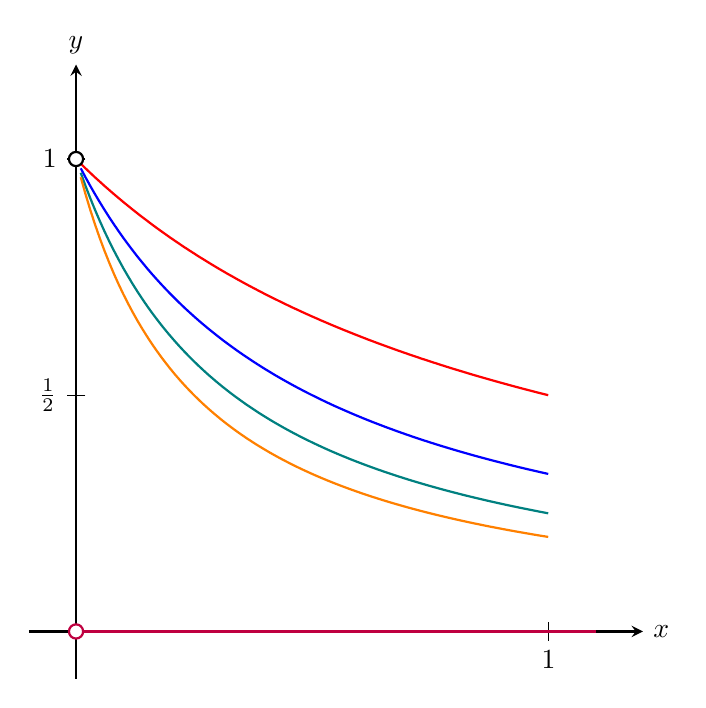
\begin{tikzpicture}[scale=6, >=stealth]
            \draw[->, thick] (-0.1, 0) -- (1.2, 0) node[right] {$x$};
            \draw[->, thick] (0, -0.1) -- (0, 1.2) node[above] {$y$};
            \draw (1, 0.02) -- (1, -0.02) node[below] {$1$};
            \draw (0.02, 1) -- (-0.02, 1) node[left] {$1$};
            \draw (0.02, 1/2) -- (-0.02, 1/2) node[left] {$\frac12$};
            \foreach \n/\col in {1/red,2/blue,3/teal,4/orange} {
                \draw[\col, thick, domain=0.01:1, samples=100]
                    plot (\x, {1/(\n*\x+1)});
            }
            \draw[purple, very thick] (0.015, 0) -- (1.1, 0);
            \filldraw[fill=white, draw=purple, thick] (0,0) circle (0.015);
            \filldraw[fill=white, draw=black, thick] (0,1) circle (0.015);
        \end{tikzpicture}
    \end{center}
\end{snippetexample}

\end{document}
